\documentclass[pdflatex,a4paper,11pt,english]{scrreprt}
\usepackage[english]{varioref}
\usepackage[utf8]{inputenc}
\usepackage[T1]{fontenc}
\usepackage{listings}
\usepackage{graphicx}
\usepackage[svgnames]{xcolor}
\usepackage[pdfborder={0 0 0}]{hyperref}
\usepackage{url}
\usepackage{array}
\usepackage{textcomp}
\usepackage[english]{babel}
\usepackage{lscape}

\clubpenalty = 10000
\widowpenalty = 10000
\displaywidowpenalty = 10000

\setcounter{secnumdepth}{3}
\setcounter{tocdepth}{4}

\begin{document}

\begin{titlepage}
\vspace*{4cm}
\begin{center}
\Large
Safety Critical Systems WS2008\\
Prof. Dr. Wagner\\
\vspace{4cm}
\normalsize
University of Applied Sciences Frankfurt\\
Faculty 2 - Computer Science and Engineering\\
M.Sc. - Program High-Integrity Systems\\
\vspace{2cm}
Insulin Pump Project\\
Documentation\\
Team 1\\
\vspace{2cm}
Wojciech Czylok, R\"udiger Gad, Elmar K\"ohler, Solomon Nega, Beril Olgun,\\
Nikolas Orlowski, Christina Paulsen, Jan Rabold, Murat Shahrashoub
\end{center}
\end{titlepage}

\tableofcontents

\listoffigures

%\lstlistoflistings

\newpage
\chapter{Project Management}
\section{Organization}

\subsection{Mindmap}
In order to get a first impression of the problem a mindmap is used (see
figure \vref{fig:mindmap}).

\begin{figure}[htb]
\centering
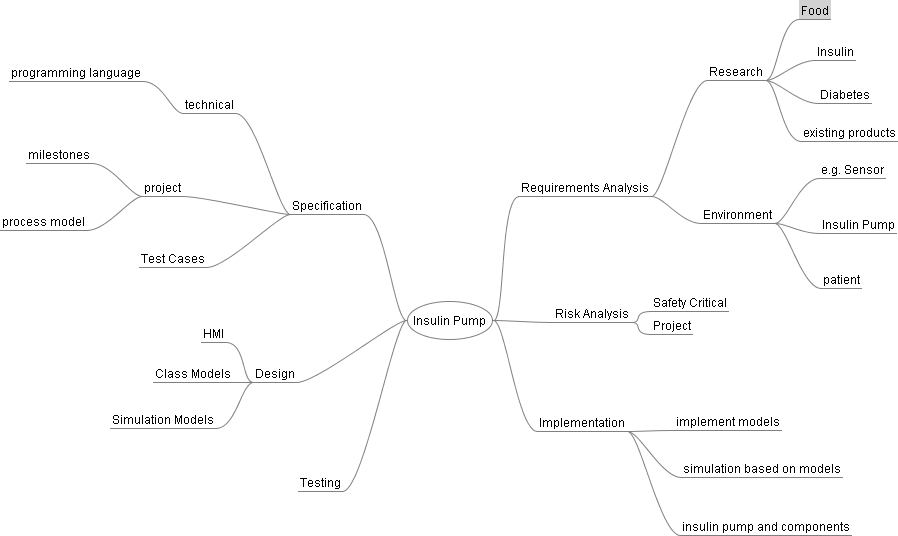
\includegraphics[width=\textwidth]{images/Insulin_Pump_Mindmap}
\caption{Mindmap of the problem}
\label{fig:mindmap}
\end{figure}

\newpage
\subsection{Development Process Model}
The spiral model is used for the main parts of our development.
See the project plan (see figures \vref{fig:projectplan1} and \vref{fig:projectplan2}) and the
mind map (see figure \vref{fig:mindmap}) for more detail.

\begin{figure}[htb]
\centering
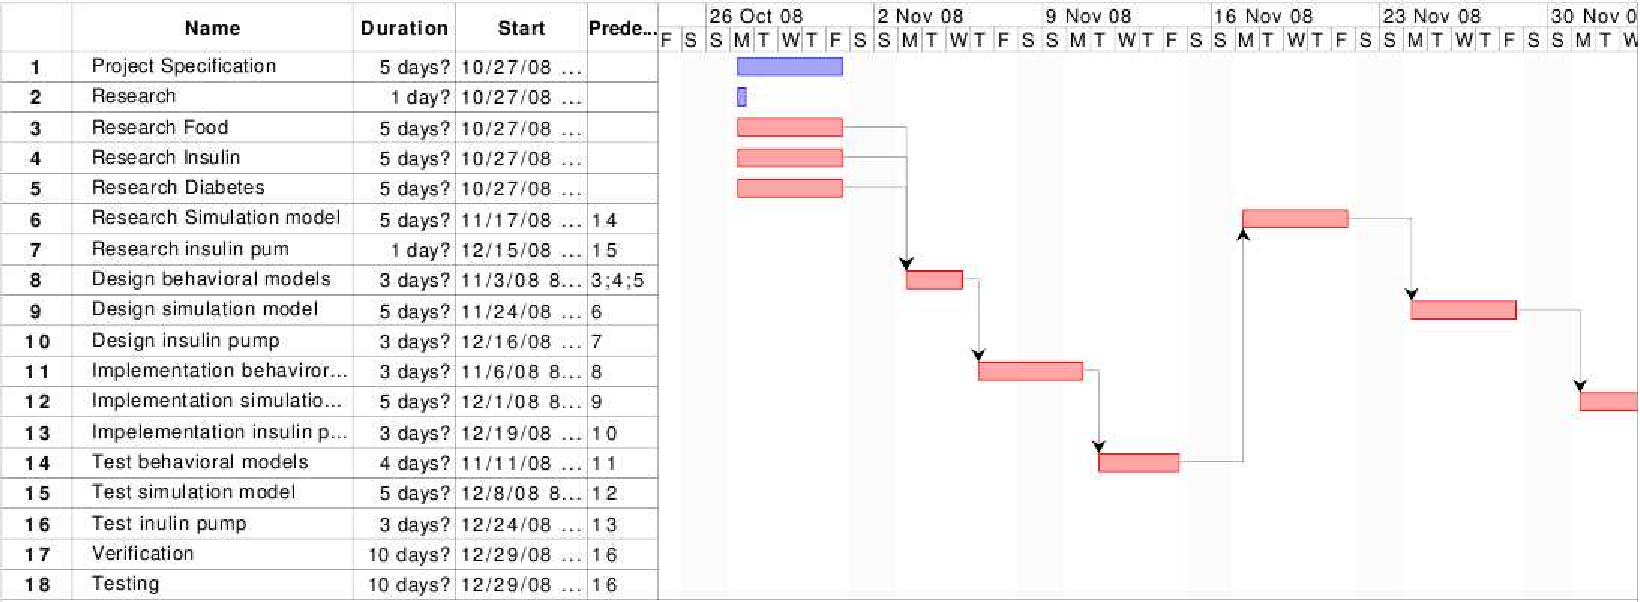
\includegraphics[width=\textwidth]{images/projectplan_page1}
\caption{Project Plan Page 1}
\label{fig:projectplan1}
\end{figure}

\begin{figure}[htb]
\centering
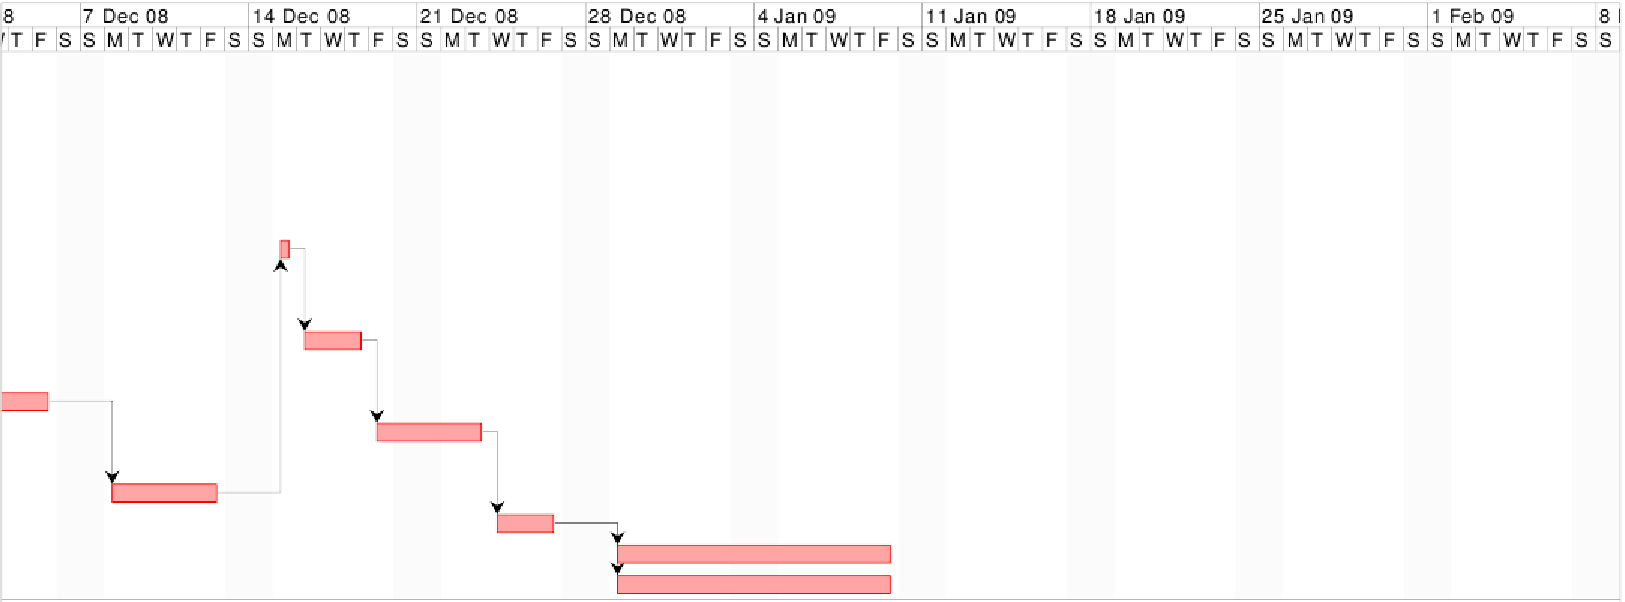
\includegraphics[width=\textwidth]{images/projectplan_page2}
\caption{Project Plan Page 2}
\label{fig:projectplan2}
\end{figure}

\newpage
At the end of November / the beginning of December quite a lot of work has
already been put into the Insulin Pump project. \\
Though it was not possible to follow the proposed project plan. \\
The following two figures show the now actual project plan (see figure
\vref{fig:projectplan_v3_1} and \vref{fig:projectplan_v3_2}):

\begin{figure}[htb]
\centering
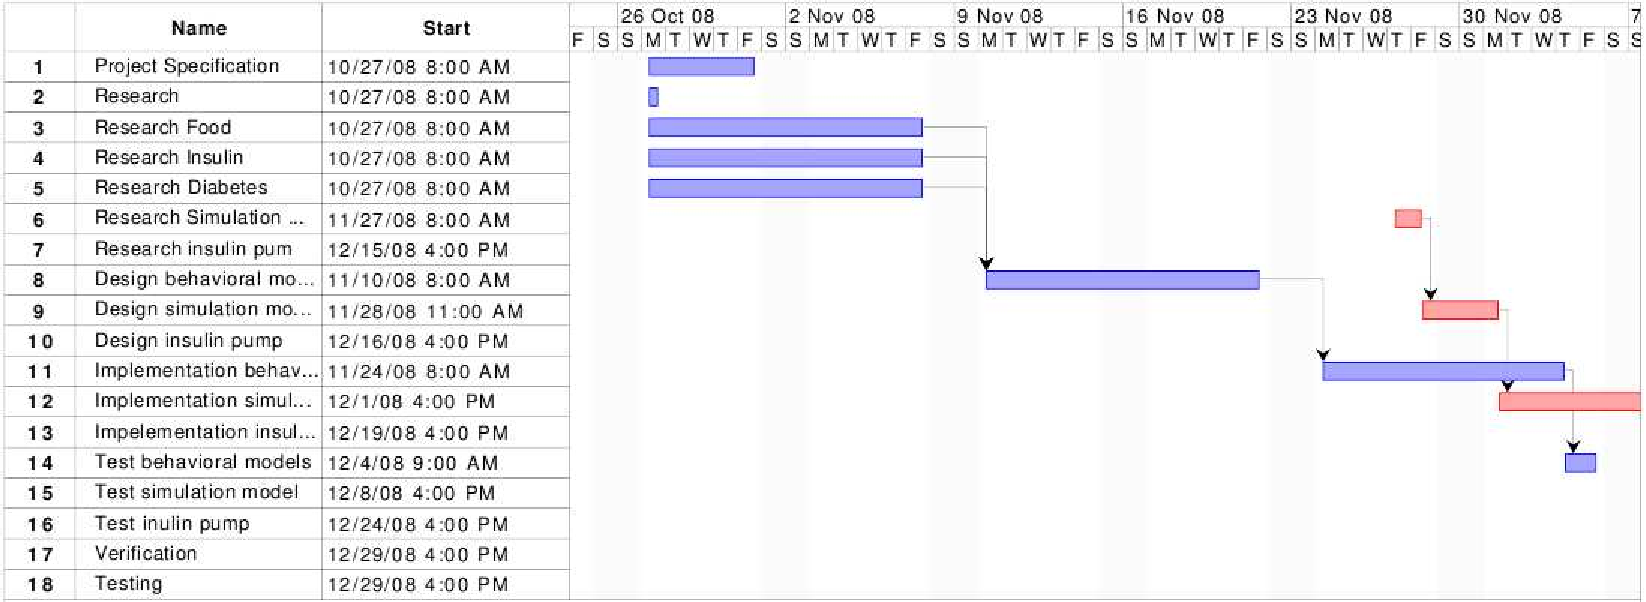
\includegraphics[width=\textwidth]{images/projectplan_v3_page1}
\caption{Project Plan (November/Dezember) Page 1}
\label{fig:projectplan_v3_1}
\end{figure}

\begin{figure}[htb]
\centering
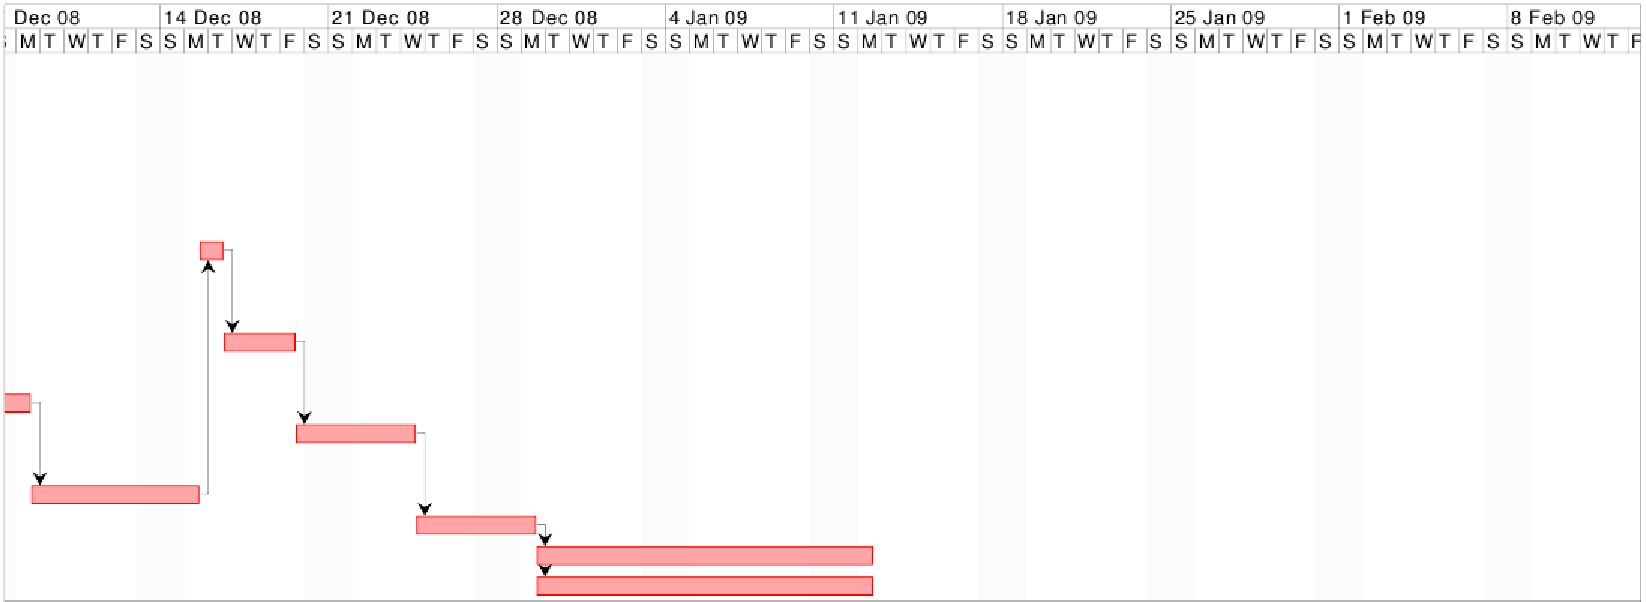
\includegraphics[width=\textwidth]{images/projectplan_v3_page2}
\caption{Project Plan (November/Dezember) Page 2}
\label{fig:projectplan_v3_2}
\end{figure}

This project plan shows now no connection from the testing of the behavioral
models to the research of the simulation.
This is because in this stage some tasks are now engaged in parallel and it was
not possible to display this in another way then this in the project plan.
This parallel process was mainly caused by different status in the groups
implementing the different behavioral models. \\
Also in order to catch up with the scheduled project plan further
simplifactions are introduced. \\
This has the purpose to deliver a working (but further simplified) product in
the end of the semester.

\subsection{Standardization}
Common value for measuring the blood glucose level is "mmol/l".
Programming language is Java.

\subsection{Specifications}
What do we want to achieve?
Simulation of the human body with diabetes and simulation of insulin pump.
Insulin pump has a sensor and automatic as well as manual injection.

\subsection{Risks}
People might get harmed or killed.
Project doesn't complete.

\subsubsection{Risk Handling}
Low glucose levels result in more serious effects on the health or even life then high levels.
So high glucose levels are prefered if there are situations when no clear preference can be made or one is in doubt.


\section{Requirements and Project Estimation}
The estimation of the project was done using COCOMO 2. Therefore the metric used here is Lines Of Code (LOC). \\ \\
First project estimation:
\begin{itemize}
  \item Behavior Simulation
  	\begin{itemize}
        \item food (Guess: 450 LOC)
        \item insulin (Guess: 400 LOC)
        \item diabetes (Guess: 400 LOC)
    \end{itemize}
  \item Simulating Insulin Pump
  	\begin{itemize}
        \item actor (Insulin injection) (Guess: 600 LOC)
        \item sensor (Glucose Level Monitor) (Guess: 150 LOC)
        \item User Interface (Alarm/Input) (Guess: 500)
    \end{itemize}
\end{itemize} 
Overall guessed LOC are 2500. \\
Guessed Estimation based on Experts Cocomo 2: \\
Effort 13.4 Person-months \\
Schedule 8.5 Months \\
\url{http://sunset.usc.edu/cgi-bin/expert_cocomo2000}

\newpage

Results from calculating metrics with "Metrics-Eclipse plugin"
\footnote{Update site for ``Metrics-Eclipse plugin''
\url{http://metrics.sourceforge.net/update}} as state of 16th of january 2009:
\begin{itemize}
  \item Behavior Simulation
  	\begin{itemize}
        \item food (LOC total 309; UI/Test ~194 LOC; Effective ~115 LOC)
        \item insulin (123 LOC)
        \item diabetes (47 LOC)
        \item model (76 LOC)
        \item view (227 LOC)
        \begin{itemize}
          \item Input (151 LOC; GUI 80 LOC; CSV 60 LOC)
          \item Output (176 LOC; GUI 114 LOC; CSV 50 LOC)
        \end{itemize}
        \item controller (141 LOC)
        \item csv (295 LOC)
    \end{itemize}
  \item Simulating Insulin Pump (Very basic implementation as of 16th of
  january 2009)
  	\begin{itemize}
        \item actor (Insulin injection) (Guess: 14 LOC)
        \item sensor (Glucose Level Monitor) (Guess: 17 LOC)
        \item User Interface (Alarm/Input) (Guess: 0 LOC (not implemented))
        \item Logic 15
    \end{itemize}
\end{itemize} 
The overall count of LOC from the computation using this module is 1390. \\
Using a different plugin (eclipsemetrics \footnote{Eclipsemetrics homepage
\url{http://www.stateofflow.com/projects/16/eclipsemetrics}}) to calculate the
total LOC the resulting value is 1191.


\chapter{Development (Body Simulation)}

\section{Requirements Analysis}
Medical Problem, Theoretic background etc.

\subsection{Research}
The research effort is split into three logical parts:
\begin{itemize}
  \item Diabetes
  \item Food
  \item Insulin
\end{itemize}
Details to the specific part of interest are explained in the following sections.

\subsubsection{Diabetes}
Diabetes mellitus, often referred to simply as diabetes, is a syndrome of disordered metabolism, usually due to a combination of hereditary and environmental causes, resulting in abnormally high blood sugar levels. 
Blood glucose levels are controlled by a complex interaction of multiple chemicals and hormones in the body, including the hormone insulin made in the beta cells of the pancreas. Diabetes mellitus refers to the group of diseases that lead to high blood glucose levels due to defects in either insulin secretion or insulin action.
\\
There are two known types of diabetes. Our Group decided to cover only diabetes type 1, because injecting of insulin is more common in this type of the disease.

\paragraph{Diabetes type 1} 
Type 1 diabetes mellitus is characterized by loss of the insulin-producing beta cells of the islets of Langerhans in the pancreas, leading to a deficiency of insulin. \\
This type of diabetes can be further classified as immune-mediated or idiopathic. The majority of type 1 diabetes is of the immune-mediated variety, where beta cell loss is a T-cell mediated autoimmune attack. \\
There is no known preventive measure which can be taken against type 1 diabetes; it is about 10\% of diabetes mellitus cases in North America and Europe (though this varies by geographical location), and is a higher percentage in some other areas. \\
Most affected people are otherwise healthy and of a healthy weight when onset occurs. Sensitivity and responsiveness to insulin are usually normal, especially in the early stages. \\
Type 1 diabetes can affect children or adults but was traditionally termed "juvenile diabetes" because it represents a majority of the diabetes cases for children. \\ \\
The principal treatment of type 1 diabetes, even in its earliest stages, is the delivery of artificial insulin via injection combined with careful monitoring of blood glucose levels using blood testing monitors. \\
Without insulin, diabetic ketoacidosis often develops which may result in coma or death. Treatment emphasis is now also placed on lifestyle adjustments (diet and exercise) though these cannot reverse the progress of the disease. \\
Apart from the common subcutaneous injections, it is also possible to deliver insulin by a pump, which allows continuous infusion of insulin 24 hours a day at preset levels, and the ability to program doses (a bolus) of insulin as needed at meal times. \\
An inhaled form of insulin was approved by the FDA in January 2006, although it was discontinued for business reasons in October 2007. [9][10] Non-insulin treatments, such as monoclonal antibodies and stem-cell based therapies, 
are effective in animal models but have not yet completed clinical trials in humans. \\ 
Type 1 treatment must be continued indefinitely in essentially all cases. Treatment need not significantly impair normal activities, if sufficient patient training, awareness, appropriate care, discipline in testing and dosing of insulin is taken. \\
However, treatment is burdensome for patients, insulin is replaced in a
non-physiological manner, and this approach is therefore far from ideal. The
average glucose level for the type 1 patient should be as close to normal
(80-120 mg/dl, 4-6 mmol/l) as is safely possible. Some physicians suggest up to
140-150 mg/dl (7-7.5 mmol/l) for those having trouble with lower values, such
as frequent hypoglycemic events. Values above 400 mg/dl (20 mmol/l) are
sometimes accompanied by discomfort and frequent urination leading to
dehydration. Values above 600 mg/dl (30 mmol/l) usually require medical
treatment and may lead to ketoacidosis, although they are not immediately
life-threatening. However, low levels of blood glucose, called hypoglycemia,
may lead to seizures or episodes of unconsciousness and absolutely must be
treated immediately, via emergency high-glucose gell placed in the patient's
mouth or an injection of glucagon.

\paragraph{Formulas} 
The calculation of absorbed insulin at a time is controlled by intervals. The pancreas produces insulin in intervals from 3-6min.
If the diabetes module indicates some new carbonates in the stomach, the total amount of needed insulin is calculated.
For 1 unit of carbonate we need 1/12 unit of insulin. Then a square function is calculated, which covers the amount of insulin needed.

\newpage
\subsubsection{Food}
There are two major "indexes" which try to relate the type of food to the foods effect on the blood sugar level (glucose level). \\
The first such index is the so called "Glycemic Index" (GI) the second one the "Glycemic Load" (GL).
The GL tries to take some criteria according to the GI in account which have been widely critizized. Still the GL and especially the GI are both still being controversially discussed by experts. \\
Most of this discussion as it appears is mainly because people tend to use
diets based on these indexes in order to try to effect blood sugar level
without medicine. \\
For a rating in a simplified simulation these indexes should
work out well, though the GL may be the one to prefer as it addresses some
weaknesses of the GI. \\
The time needed for food to affect the blood sugar can roughly be splitted up
into three groups of food which affect blood sugar level fast, moderate or
slowly.

\paragraph{Simulation} 
In order to simulate the glucose level increase, after food has been eaten, programatically, mathematical models have to be made in order to calculate this process. \\
Here it is focused on the three main types of different types of food with respect to speed of their absorbtion (i.e. how fast the gluscose level rises after a meal). \\
These three main types split up in

\begin{itemize}
  \item high glycemic (fast),
  \item moderate glycemic (intermediate) and
  \item low glycemic (slow) foods.
\end{itemize}

Unfortunately there are no mathematical models available for simulating this.
So in order to make a somewhat sane simulation there is the suggestion to use different formulas in order to simulate the different behavior of these food types. The type of formula choosen should represent the behavior of glucose level absorbtion / increase in an approximate way. The ammount of the glucose increases and roughly the timespan it occours in can be influenced by variables in these formulas. \\
Fortunately at least rough estimates can be made according to the absorbtion of
glucose in the blood as there exists a table which associates different food types
with their behavior according to CI, CL etc.

\newpage

\paragraph{Formulas} 
So far two formulas have been evaluated. \\
Formula a (see figure \vref{fig:food_function_a}) has no skew and therefore is
symmetric. 

\begin{figure}[htb]
\centering
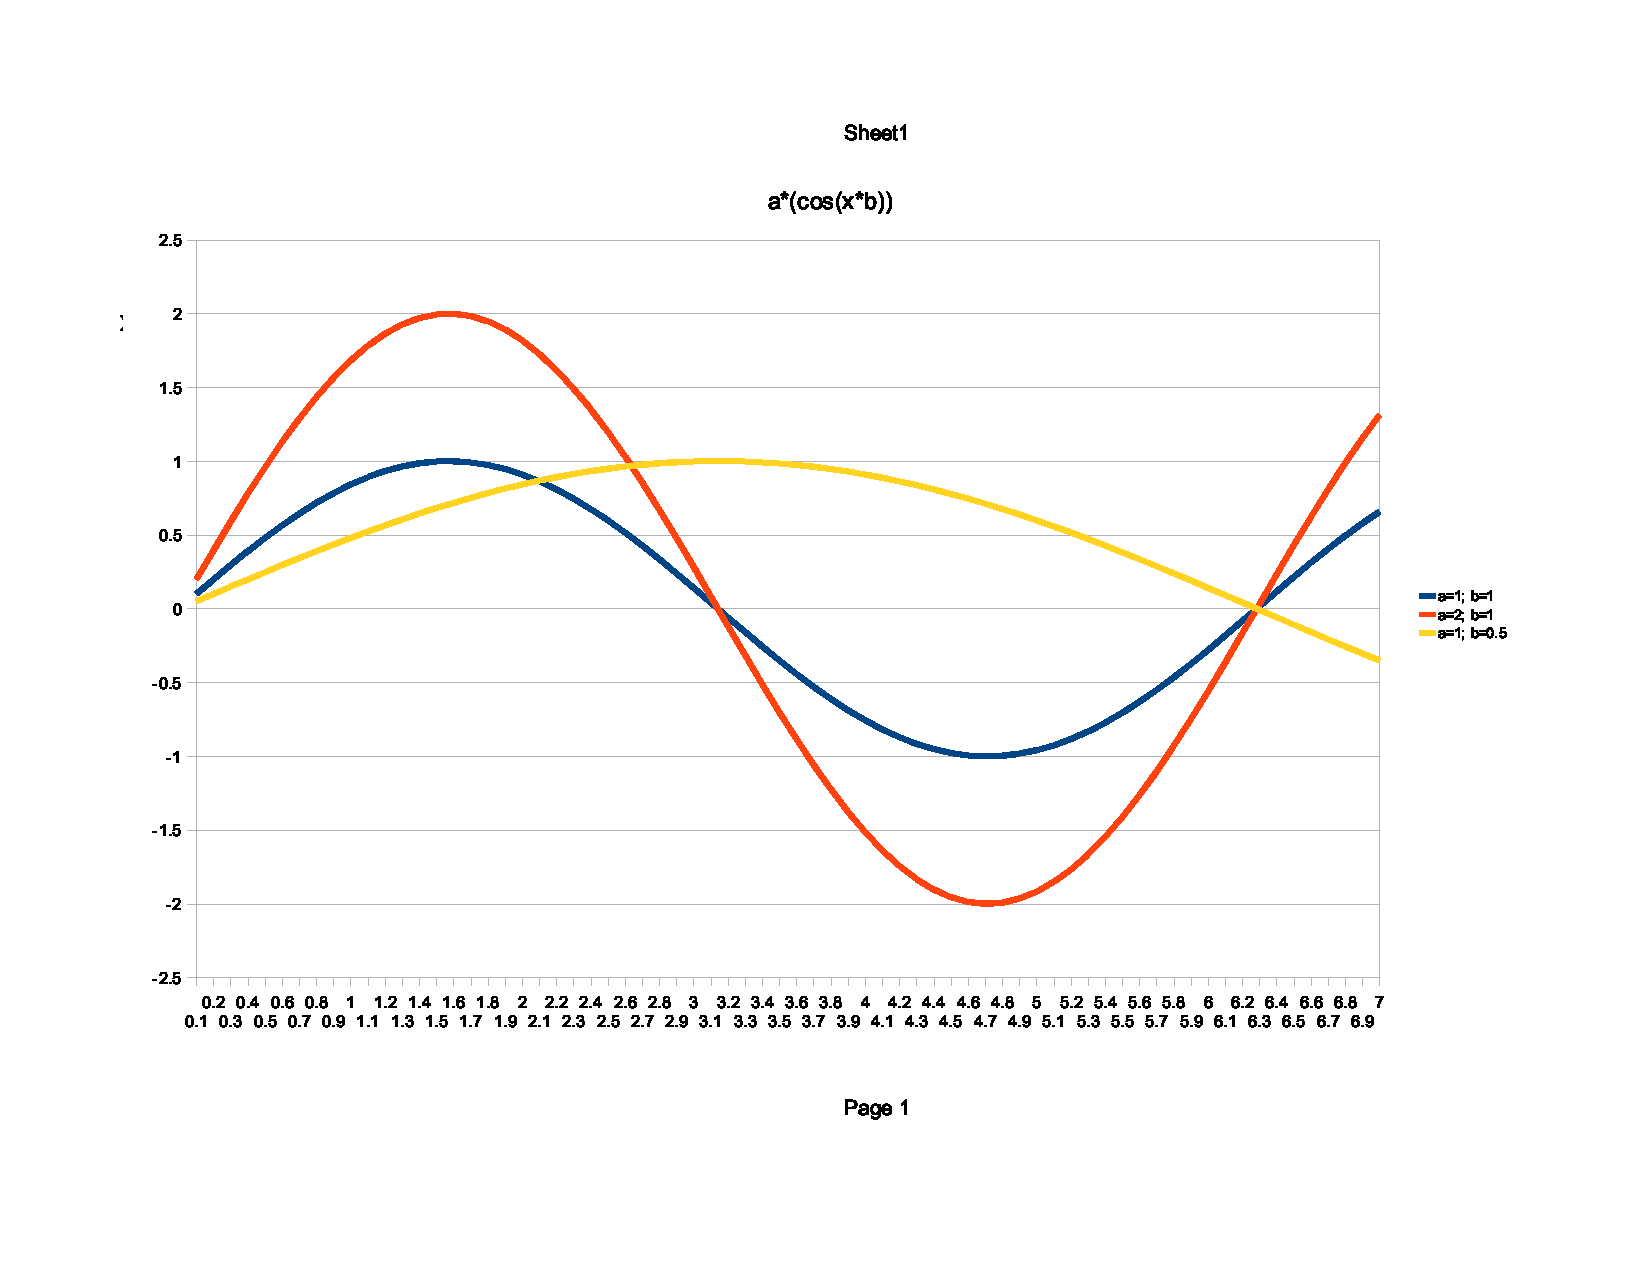
\includegraphics[scale=0.4]{images/food_function_a}
\caption{Food Function A}
\label{fig:food_function_a}
\end{figure}

\newpage

Formula b (see figure \vref{fig:food_function_b}) has a skew to the right. I.e.
it increases "slowly" two some point from which on it falls very abruptly. 

\begin{figure}[htb]
\centering
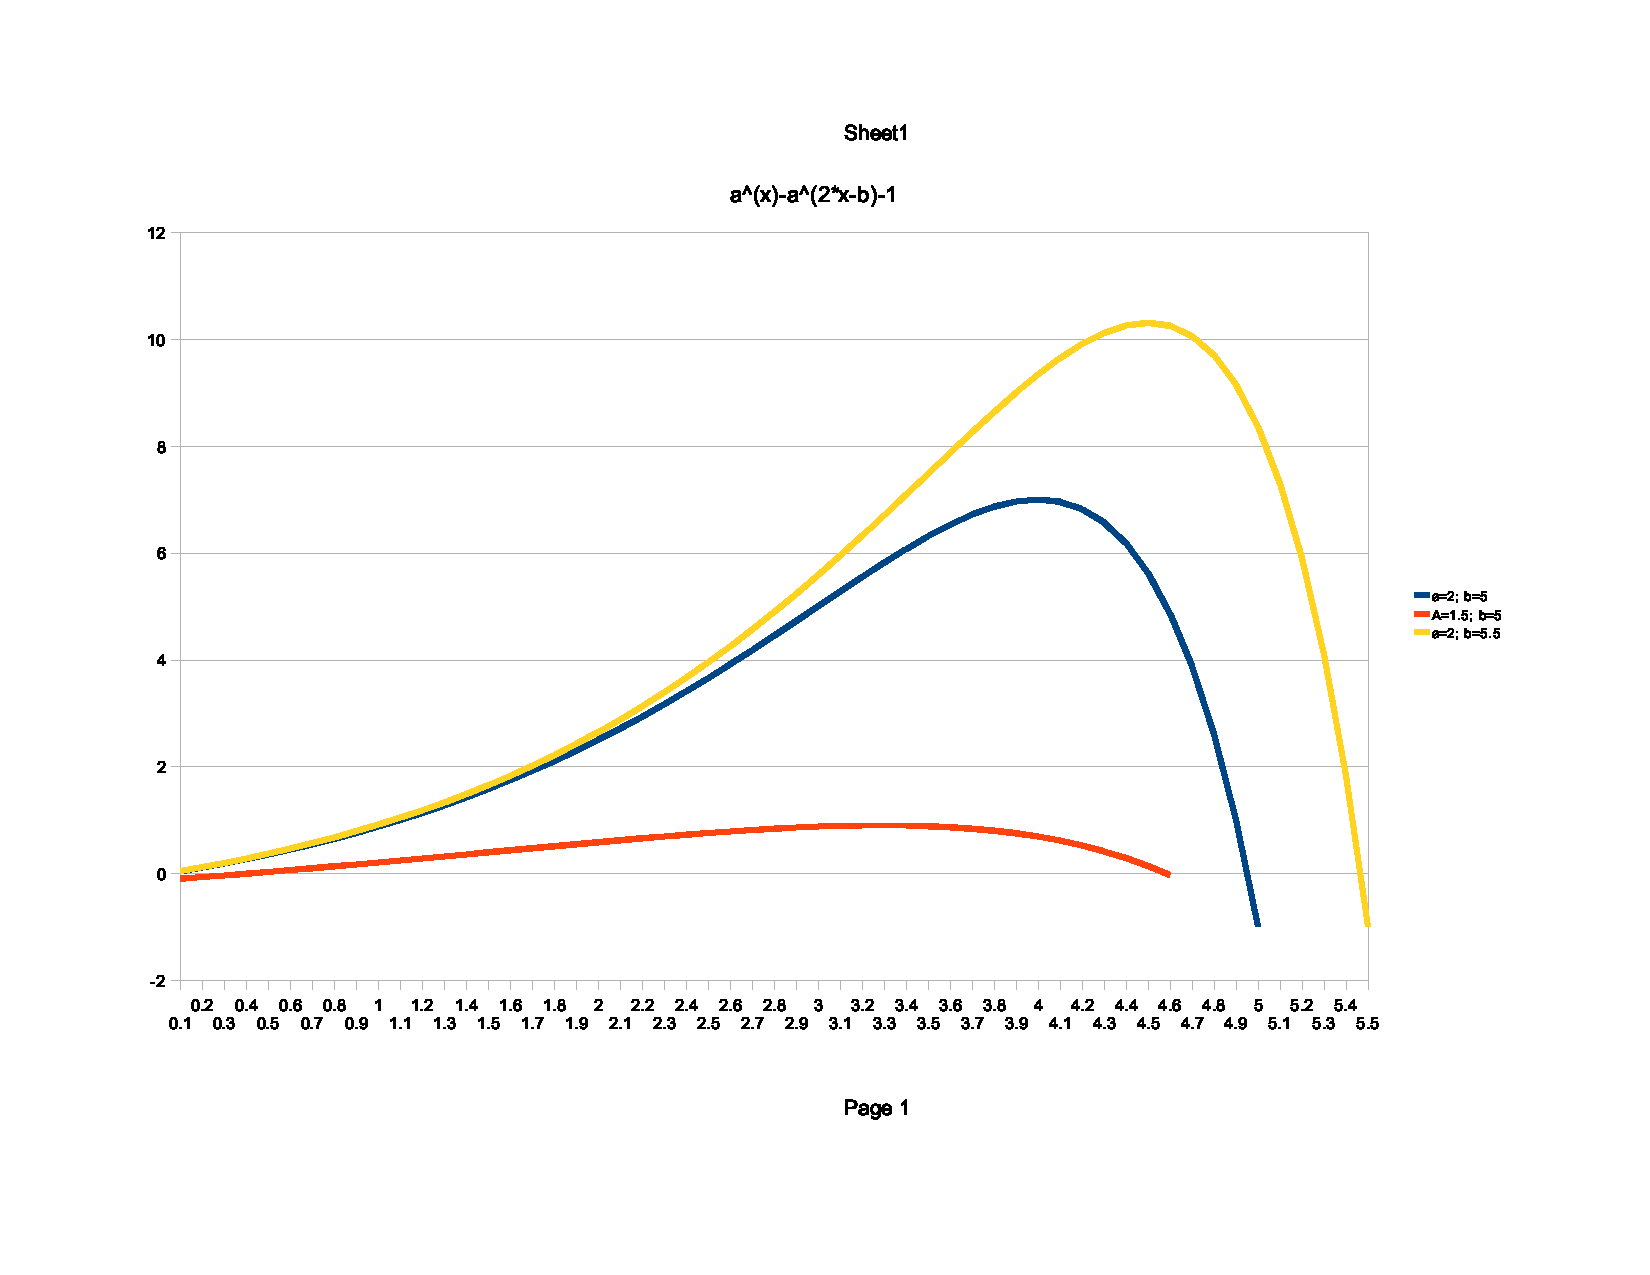
\includegraphics[scale=0.4]{images/food_function_b}
\caption{Food Function B}
\label{fig:food_function_b}
\end{figure}

\paragraph{Implementation} 
In order to make it more flexible to choose different algorithms / formulas for
calculating the glucose values the Strategy pattern might be choosen. One
critical question with respect to the implementation is the choice of the used
data types for floatingpoint data as these data types are not guaranteed to be precise.

\newpage

\subsubsection{Insulin}

\begin{figure}[htb]
\centering
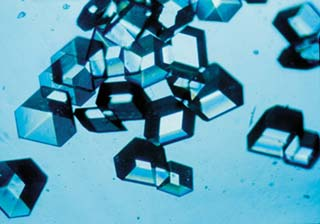
\includegraphics[scale=0.4]{images/Insulincrystals}
\caption{Insulin crystals}
\end{figure}
Insulin is a hormone, which is produced in the beta-cells of the pancreas and it's essential for humans and animals. 
Taking of insulin causes decreasing of the blood glucose level and consuming glucagon or energy source. 
Glucagon and some other hormones (e.g. adrenaline, cortisone and pancreas hormones) will increase the blood glucose level.\\

In addition some other properties:
\begin{itemize}
  \item after ingestion of carbohydrates the blood glucose level will be increased, 
	  therefore insulin will be degraded to terminate this process
  \item if fats and proteins are eaten at the same time as carbohydrates, 
	  then it will cause delays in absorption of glucose
  \item differences in the absorption speed of glucose between foods with the same amount
  \item movement reduces the need of insulin
\end{itemize}

\newpage

\paragraph {Types}
There are some commonly used types of insulin: \\

\begin{tabular}{lcr}
	\textbf{Synonym} & \textbf{Starts working} & \textbf{Duration}\\
	Insulin analogs (rapid-acting) & 5 to 15 minutes & 3 to 4 hours\\
	Regular insulin(short-acting) & approx. 30 minutes & 5 to 8 hours\\
	Semilente insulin (intermediate-acting) & 1 to 3 hours & 16 to 24 hours\\
	Ultralente insulin (long-acting) & 4 to 6 hours & greater than 32 hours\\
	Insulin glargine/ detemir & 1 to 2 hours & approx. 24 hours\\
	Mixture of NPH and regular insulin & approx. 30 minutes & 16 to 24 hours\\
	Mixture of semilente and ultralente & ? & 24 hours\\
\end{tabular}

\paragraph{Dosage and Timing}
Usually insulin is released into the blood every 3 to 6 minutes. The central problem is to pick the right dose of insulin and the right timing. The following diagram shows a plan of the glucose- and insulin levels during the day.

\begin{figure}[htb]
\centering
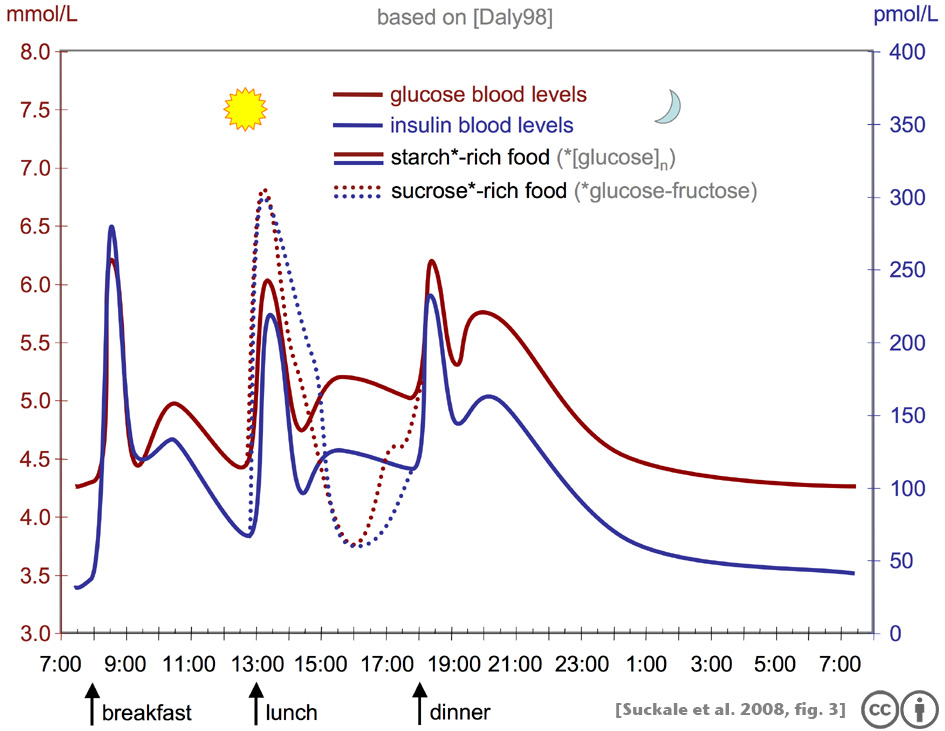
\includegraphics[width=\textwidth]{images/Suckale08_fig3_glucose_insulin_day}
\caption{Influences of the blood glucose- and insulin level}
\end{figure}

It is impossible to know how much insulin is needed for an optimum blood glucose level, because of the complex and 
interacting factors. For example some patients with diabetes require more insulin after drinking skim milk than 
they do after taking an equivalent amount of fat, protein, carbohydrate, and fluid in some other form.\\

\paragraph{Strategies}

\begin{itemize}
  \item Long-acting insulin will be used for the approximate release of the pancreas (NPH, ultralente, glargine, detemir)
  \item Short-acting insulin will be used for the anticipation of eating (insulin analogs like lispro, aspart and 
	  glulisine can be used while- or after eating, regular insulin has to be used 30 minutes before eating)
  \item The blood glucose level has to be checked before all meals and sometimes also at bedtime
  \item Some guidelines call for check 2 hours after a meal
\end{itemize}

mmol/l <-> mg/dl convertion ; hypoglycemia \& hyperglycemia (Table)\\

\begin{description}
  \item[Red values of blood sugar (hypoglycemia)] The blood sugar is too deep. With progressive drop the blood sugar mirror, the diabetic can fall in coma.
  \item[Green values of blood sugar] Blood sugar within the desirable range. Normal values.
  \item[Turquoise values of blood sugar] The blood sugar is easily increased. (offen after a meal). With a person without diagnosed diabetes further is it necessary to check blood-measurements and to diagnose the diabetes.
  \item[Blue values of blood sugar (hyperglycemia)] Blood sugar values are clearly too high. Non-diabetic should visit the doctor. 
He must be classfy, if he gotten sick. A diabetic must inject immediately fast-effective correction insulin. 
With further blood sugar rising is it possible to get the dangerous coma.
\end{description}

\begin{figure}[htb]
\centering
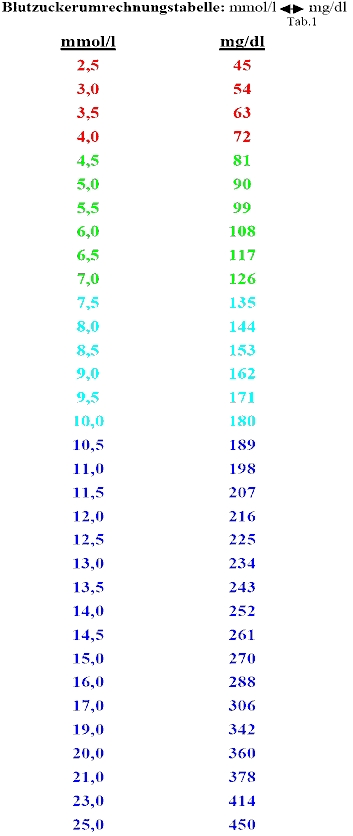
\includegraphics[scale=0.6]{images/Conversion}
\caption{Blood glucose levels}
\end{figure}

\paragraph{Existing products} 
Most insulin products give information about the duration and starting time. The glucose blood level differs from human to human, therefore it's difficult to define the effect of the injected insulin. 
Normal blood sugar values are from 4,5 to 7,0 mmol/L and we assume that it's possible to inject max. 12 units insulin at once and normally an average of 5 units.\\

\newpage

\textbf{The effect of one unit insulin?}

\begin{figure}[htb]
\centering
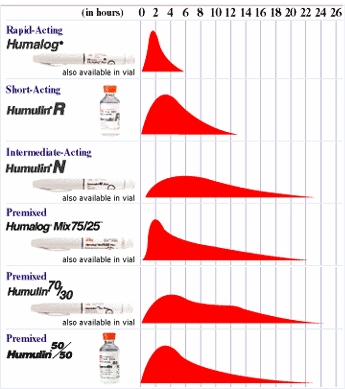
\includegraphics[scale=1]{images/time_activity}
\caption{Durations of different Canine Insulin types}
\end{figure}


\section{List of Requirements}
Requirement specification \\
The overall goal of the project is to simulate
\begin{itemize}
  \item the human body with the illness diabetes and the aspects introduced
  by this illness as well as the reaction on food and insulin injection
  \item an insulin pump which reacts on the behavior of the the above given
  simulation of the human body with the illness diabetes.
\end{itemize}

The first step therefore is to provide a simulation of the human body with the
illness diabetes and the aspects food and insulin. \\ 
Since this is quite a big task it is divided into modules. These modules should
first on their own simulate the behavior of diabetes, food and insulin and are
therefore called behavioral modules.

\subsection{Behavioral Modules}

\subsubsection{Diabetes Module}
\paragraph{Simulation} 
The diabetes module needs to simulate the insulin production of an ill pancreas. 
As an indicator the module needs the amount of carbonate in the stomach and the time of calculation.

\subsubsection{Food Module}
For reasons of simplification only the three major food groups are taken into
account.\\
These groups are 
\begin{itemize}
  \item high glycemic (fast),
  \item moderate glycemic (intermediate) and
  \item low glycemic (slow) foods.
\end{itemize}
In order to provide means to calculate the behavior of these groups
mathematical models need to be developed and / or researched to allow the
simulation.

\subsubsection{Insulin Module}
There are many insulin types, because of the given possibility to mix different 
insulin types together. Therefore we decided to implement the following three types of insulin:

\begin{itemize}
   \item Rapid-Acting
   \item Short-Acting
   \item Long-Acting
\end{itemize}

The different properties of each type are described in chapter 2.1.1.3!

\subsection{Body Simulation}
The body simulation combines all behavioral modules and therefore simulates the
behavior of the human body with the illness diabetes.\\ \\
Inputs of this body simulation are food and insulin. \\
Outputs are glucose and insulin values over time. \\ \\

Concrete requirements are as follows:
\begin{itemize}
  \item Inputs must be realized as GUI and as inputs via given CSV-Files.
  \item Outputs must be realized as GUI and as CSV-Files.
  \item The behavioral modules created in the first step are combined to one
  large model.
\end{itemize} 

\subsection{Test Cases}
Test cases need to be designed for the complete simulation but as well for the
smaller parts (e.g. behavioral modules etc.).


\newpage

\section{Analysis Models}
These models serve as conceptual designs and are later used when it comes to
concrete implementations.

\subsection{Behavioral modules and interaction}

\begin{figure}[htb]
\centering
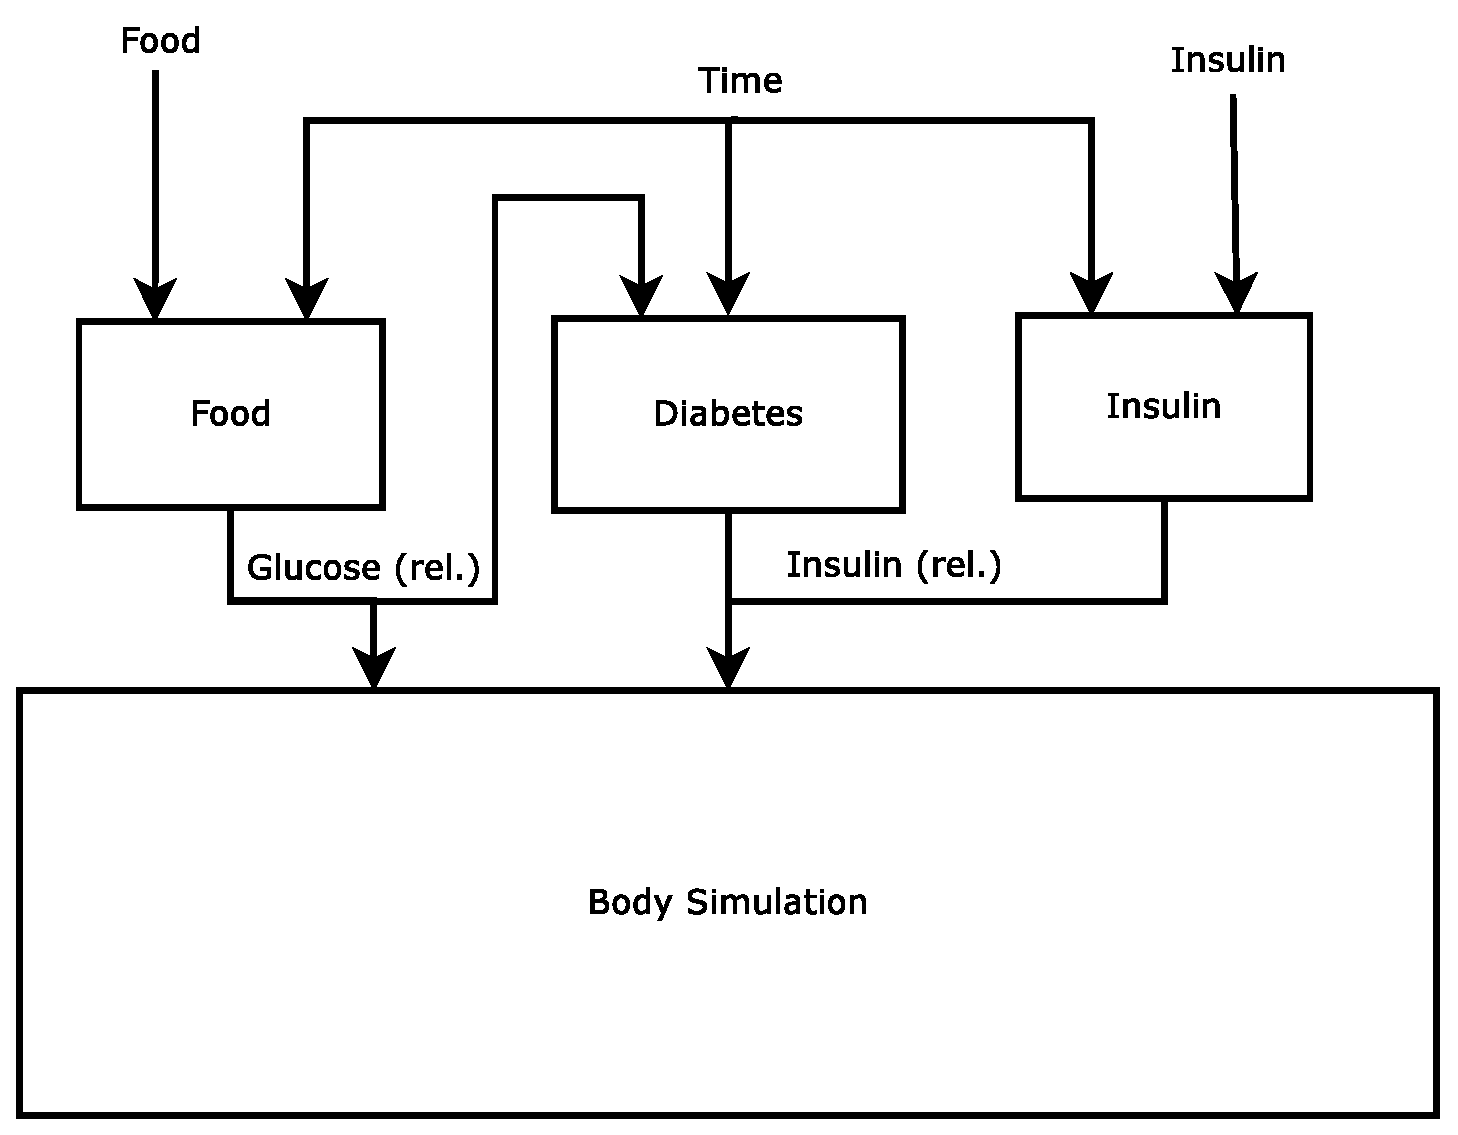
\includegraphics[scale=0.4]{images/Analysis_Model}
\caption{Analysis model of behavioral modules and theire interaction}
\label{fig:analysis_model_behavioral_modules}
\end{figure}

\newpage
\subsection{Body simulation (aka: putting behavioral modules together)}
The body simulation must combine the three behavioral modules and provide
inputs and outputs to these.
Such in- and outputs include but are not limited to GUIs and reading/writing
from/to CSV-Files. \\
A first conceptual design can look as follows (see
\vref{fig:body_sim_analysis_model}):

\begin{figure}[htb]
\centering
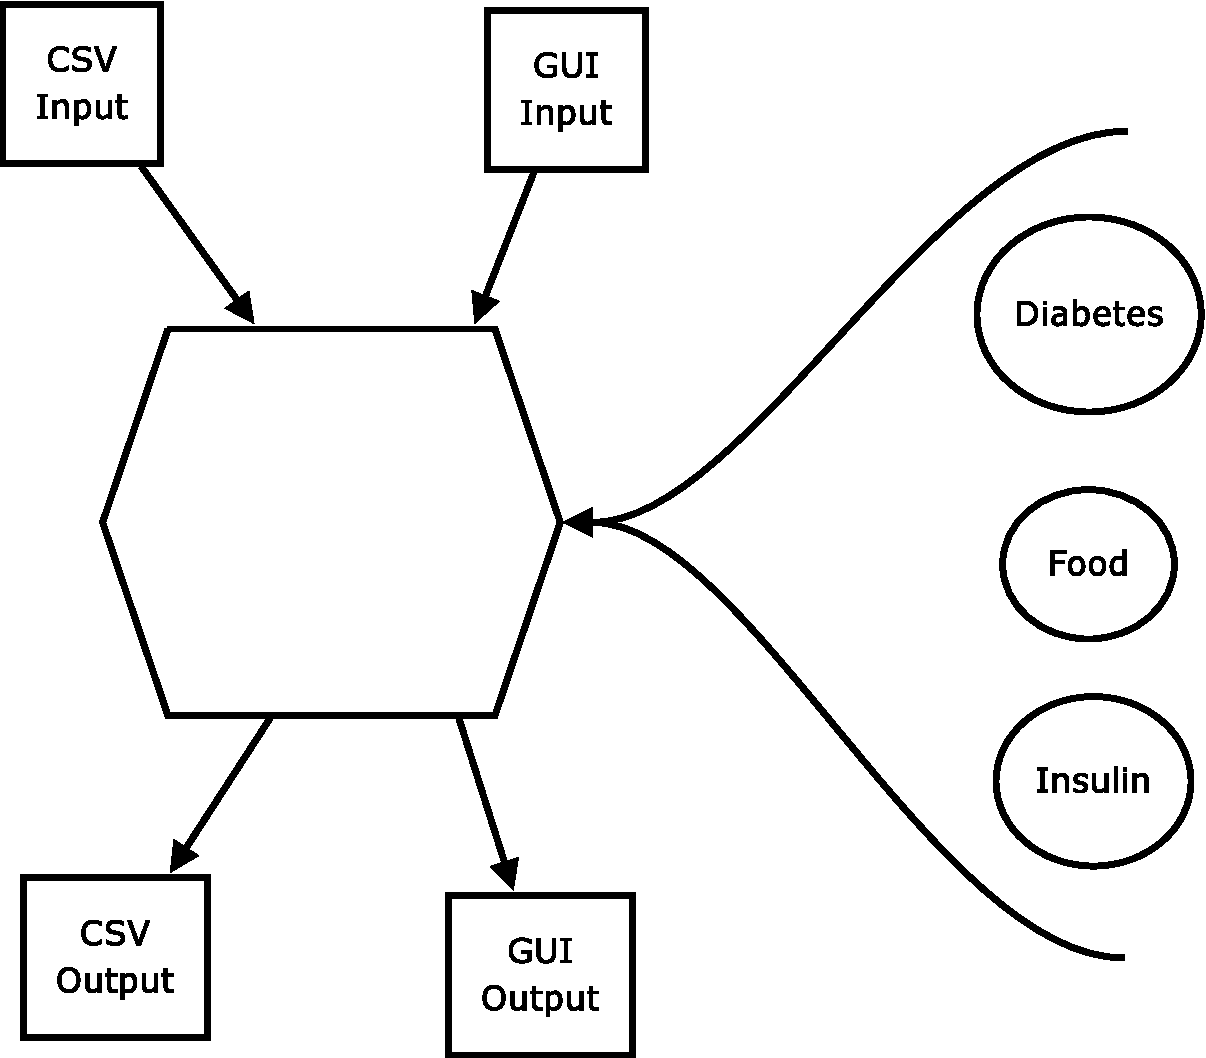
\includegraphics[scale=0.4]{images/Body_Simulation_analysis_model}
\caption{Body simulation analysis model}
\label{fig:body_sim_analysis_model}
\end{figure}

\newpage
\section{Design Models}
These models represent the concrete class diagrams which are planned and are to
be implemented. 

\subsection{Behavioral Modules}
For the Behavioral Modules we decided to show the Food Module as an example:


\subsubsection{Food}
In order to provide the possibility for extensive and intuitive testing for the
food module also some GUI components have been designed. These components include a frontend for input (e.g. adding food to the simulation etc.) and a display of the output. \\
In order to provide large flexibility with respect to future changes the
concrete food types inherit from an abstract class. This way it is possible to
program to an abstraction (the abstract class) rather then implementations (the
subclasses inheriting from the abstract class). \\
Fulfilling this design principle provides large flexibiltiy when new (e.g. more
finely grained behaving) food implementations should be realized.\\
The update of the output display is implemented using the Observer Pattern.
With the output "ChartDisplay" being the observer of the `"FoodModule".
\\
The resulting class diagram is as follows (see
\vref{fig:food_module_class_diagram}):

\begin{figure}[htb]
\centering
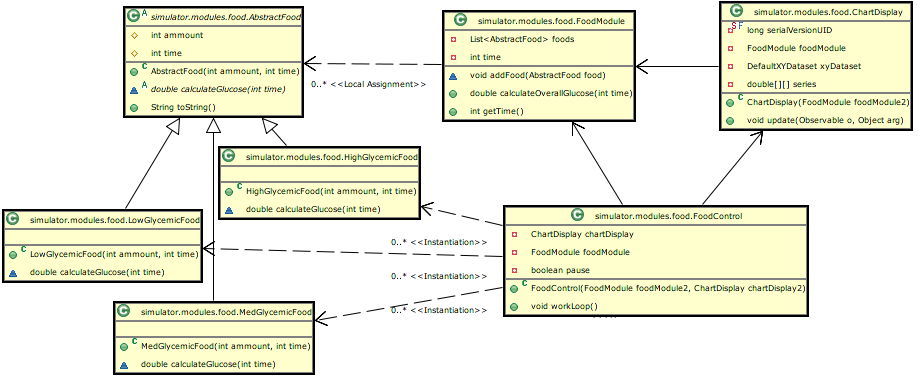
\includegraphics[width=\textwidth]{images/food_module_class_diagram2}
\caption{Food Module Class Diagram}
\label{fig:food_module_class_diagram}
\end{figure}


\newpage
\subsection{Body Simulation}
\label{sec:body_simulation}
For implementing the body simulation and putting all the behavioral modules
together while still providing large flexibility for further extensions and
changes the Model View Controller paradigm is used (see figure
\vref{fig:mvc_simplified}). 

\begin{figure}[htb]
\centering
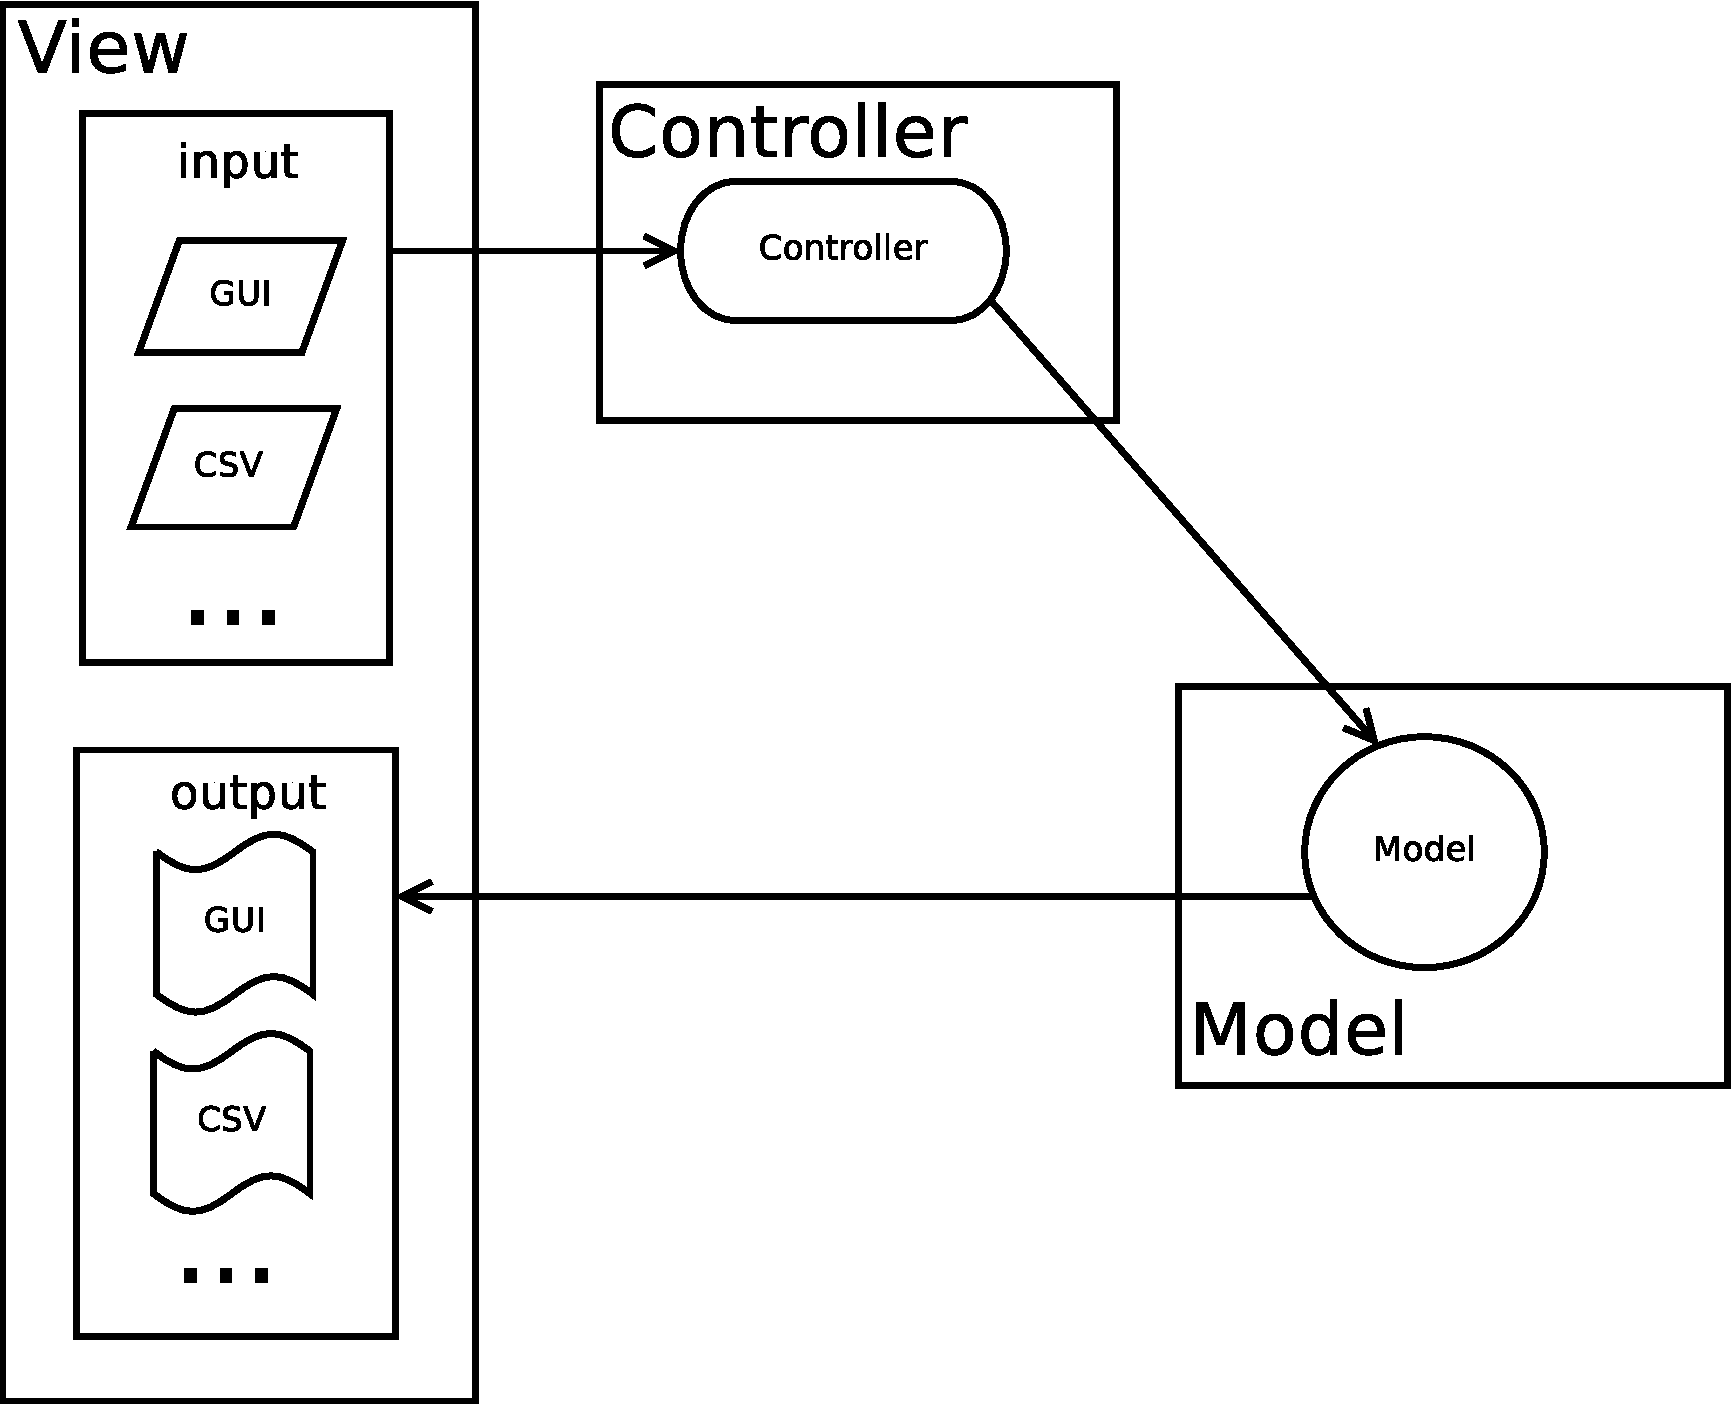
\includegraphics[scale=0.4]{images/mvc_simplified}
\caption{Simplified illustration of Model View Controller concept}
\label{fig:mvc_simplified}
\end{figure}

This should also allow an easy integration of the components of the insulin pump which interact with the human body (i.e. sensor and injection unit). \\
The resulting class design is as follows  (see figure
\vref{fig:body_simulation_class_diagram}): 

\begin{landscape}
\begin{figure}[htb]
\centering
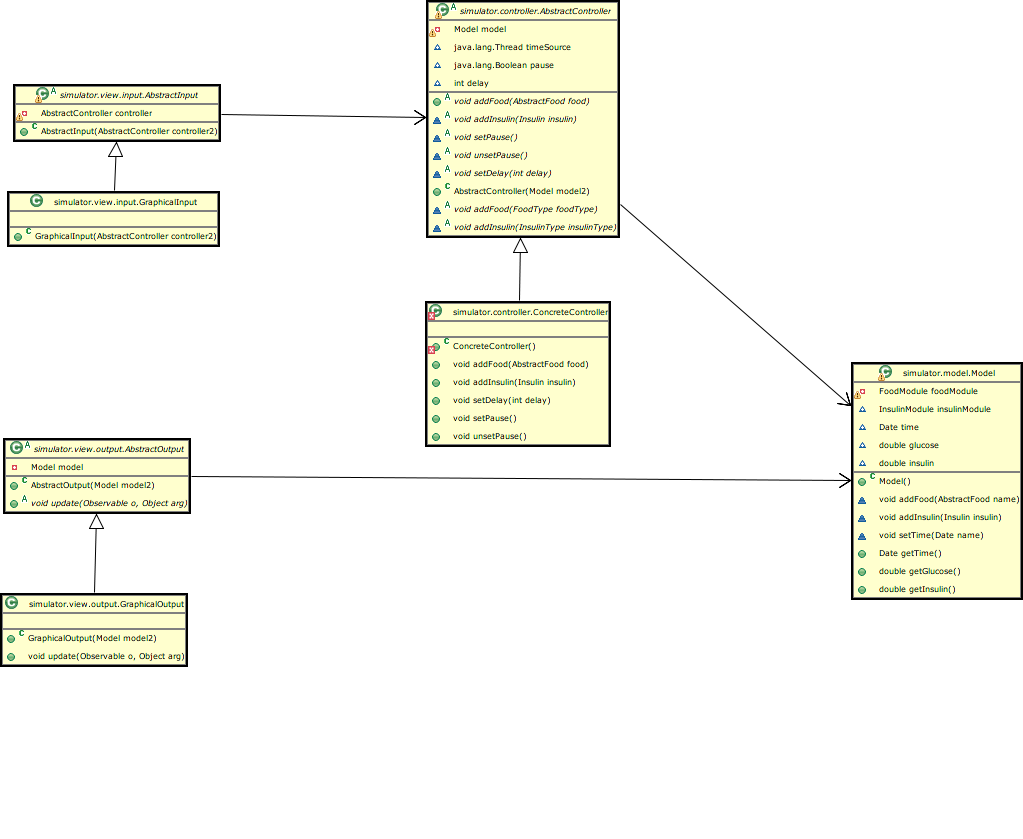
\includegraphics[width=\textwidth]{images/body_simulation_classdiagram}
\caption{Body Simulation Class Diagram}
\label{fig:body_simulation_class_diagram}
\end{figure}
\end{landscape}


\chapter{Development (Insulin Pump)}

\section{Research}
First a list of available information that can be achieved from the
mesurement:
\begin{itemize}
  \item the glucose level
  \item the time difference between now and the previous injections
  \item the gradient of the glucose curve at the time of the current measurement
  \item the insulin that will be available in the period p which can be
  calculated as now + "length of p" (p can be e.g. 1, 2, 5, 10, 30, \ldots
  minutes or 1, 2, 5, 10, \ldots hours)
  \item the average of the glucose level since a defined point t in the past (t
  has the same definition as p)
\end{itemize}

\subsection{Calculation steps}

\subsubsection{Calculate the gradient (GR) for the current timestamp}
Because of the reason that we don't have the function of the glucose curve we need to calculate the gradient. One way is to take the gradient from the last and the actual measurement.

\subsubsection{Calculate the available insulin (IN)}
The available insulin can be calculated like in the simulation that you take
the actual timestamp and simply add a period to this time. With the new
timestamp the module insulin and the module pangria can calculate the available
insulin for a given period in the future.

\subsubsection{Calculate the actual needed amount of insulin}
As higher GR is as longer the insulin level would increase. Then much more
insulin is needed to get the level down to normal. Then we can calculate with
the amount that is needed to get the glucose level to normal and subtract (IN)
from this. The result (RE) can be injected. \\
This is a very simple attempt to calculate the needed amount of insulin. \\ \\
It can be assumed that it is possible to set a static amount of insulin
that will be given by the pangria - in order to keep the simplicity for this project. This static amount will be included in the calculation.

\subsection{Further Thoughts}
\begin{itemize}
  \item It is possible to put a factor in front of RE so that just a part of
  the insulin will be injected. The factor depends on GR.
  \item We should think about the time period between the measurements to the
  best result.
  \item We should define some levels where we put some extra insulin to avoid
  peaks e.g. if we have a big GR but we were in the dangerous area (too less
  sugar then it's a problem but if we are in an area where we are already too
  high than it is very dangerous).
  \item It is possible not to calculate the amount for the future but for the
  past so that we could say in the last period the amount of glucose increased by
  "x" and how much insulin is needed to absorb the glucose.
  \item In some way we should have a warning in the pump where we inform the
  user if he is in the dangerous area (too high or too low).
\end{itemize}

\section{Analysis Model}

\section{Design Model}
Thanks to the very open and flexible implementation of the Body Simulation
following the Model View Controller (see section \vref{sec:body_simulation})
paradigm, the sensor and injector components of the Insulin pump can be very
easily integrated into the model.

\begin{figure}[htb]
\centering
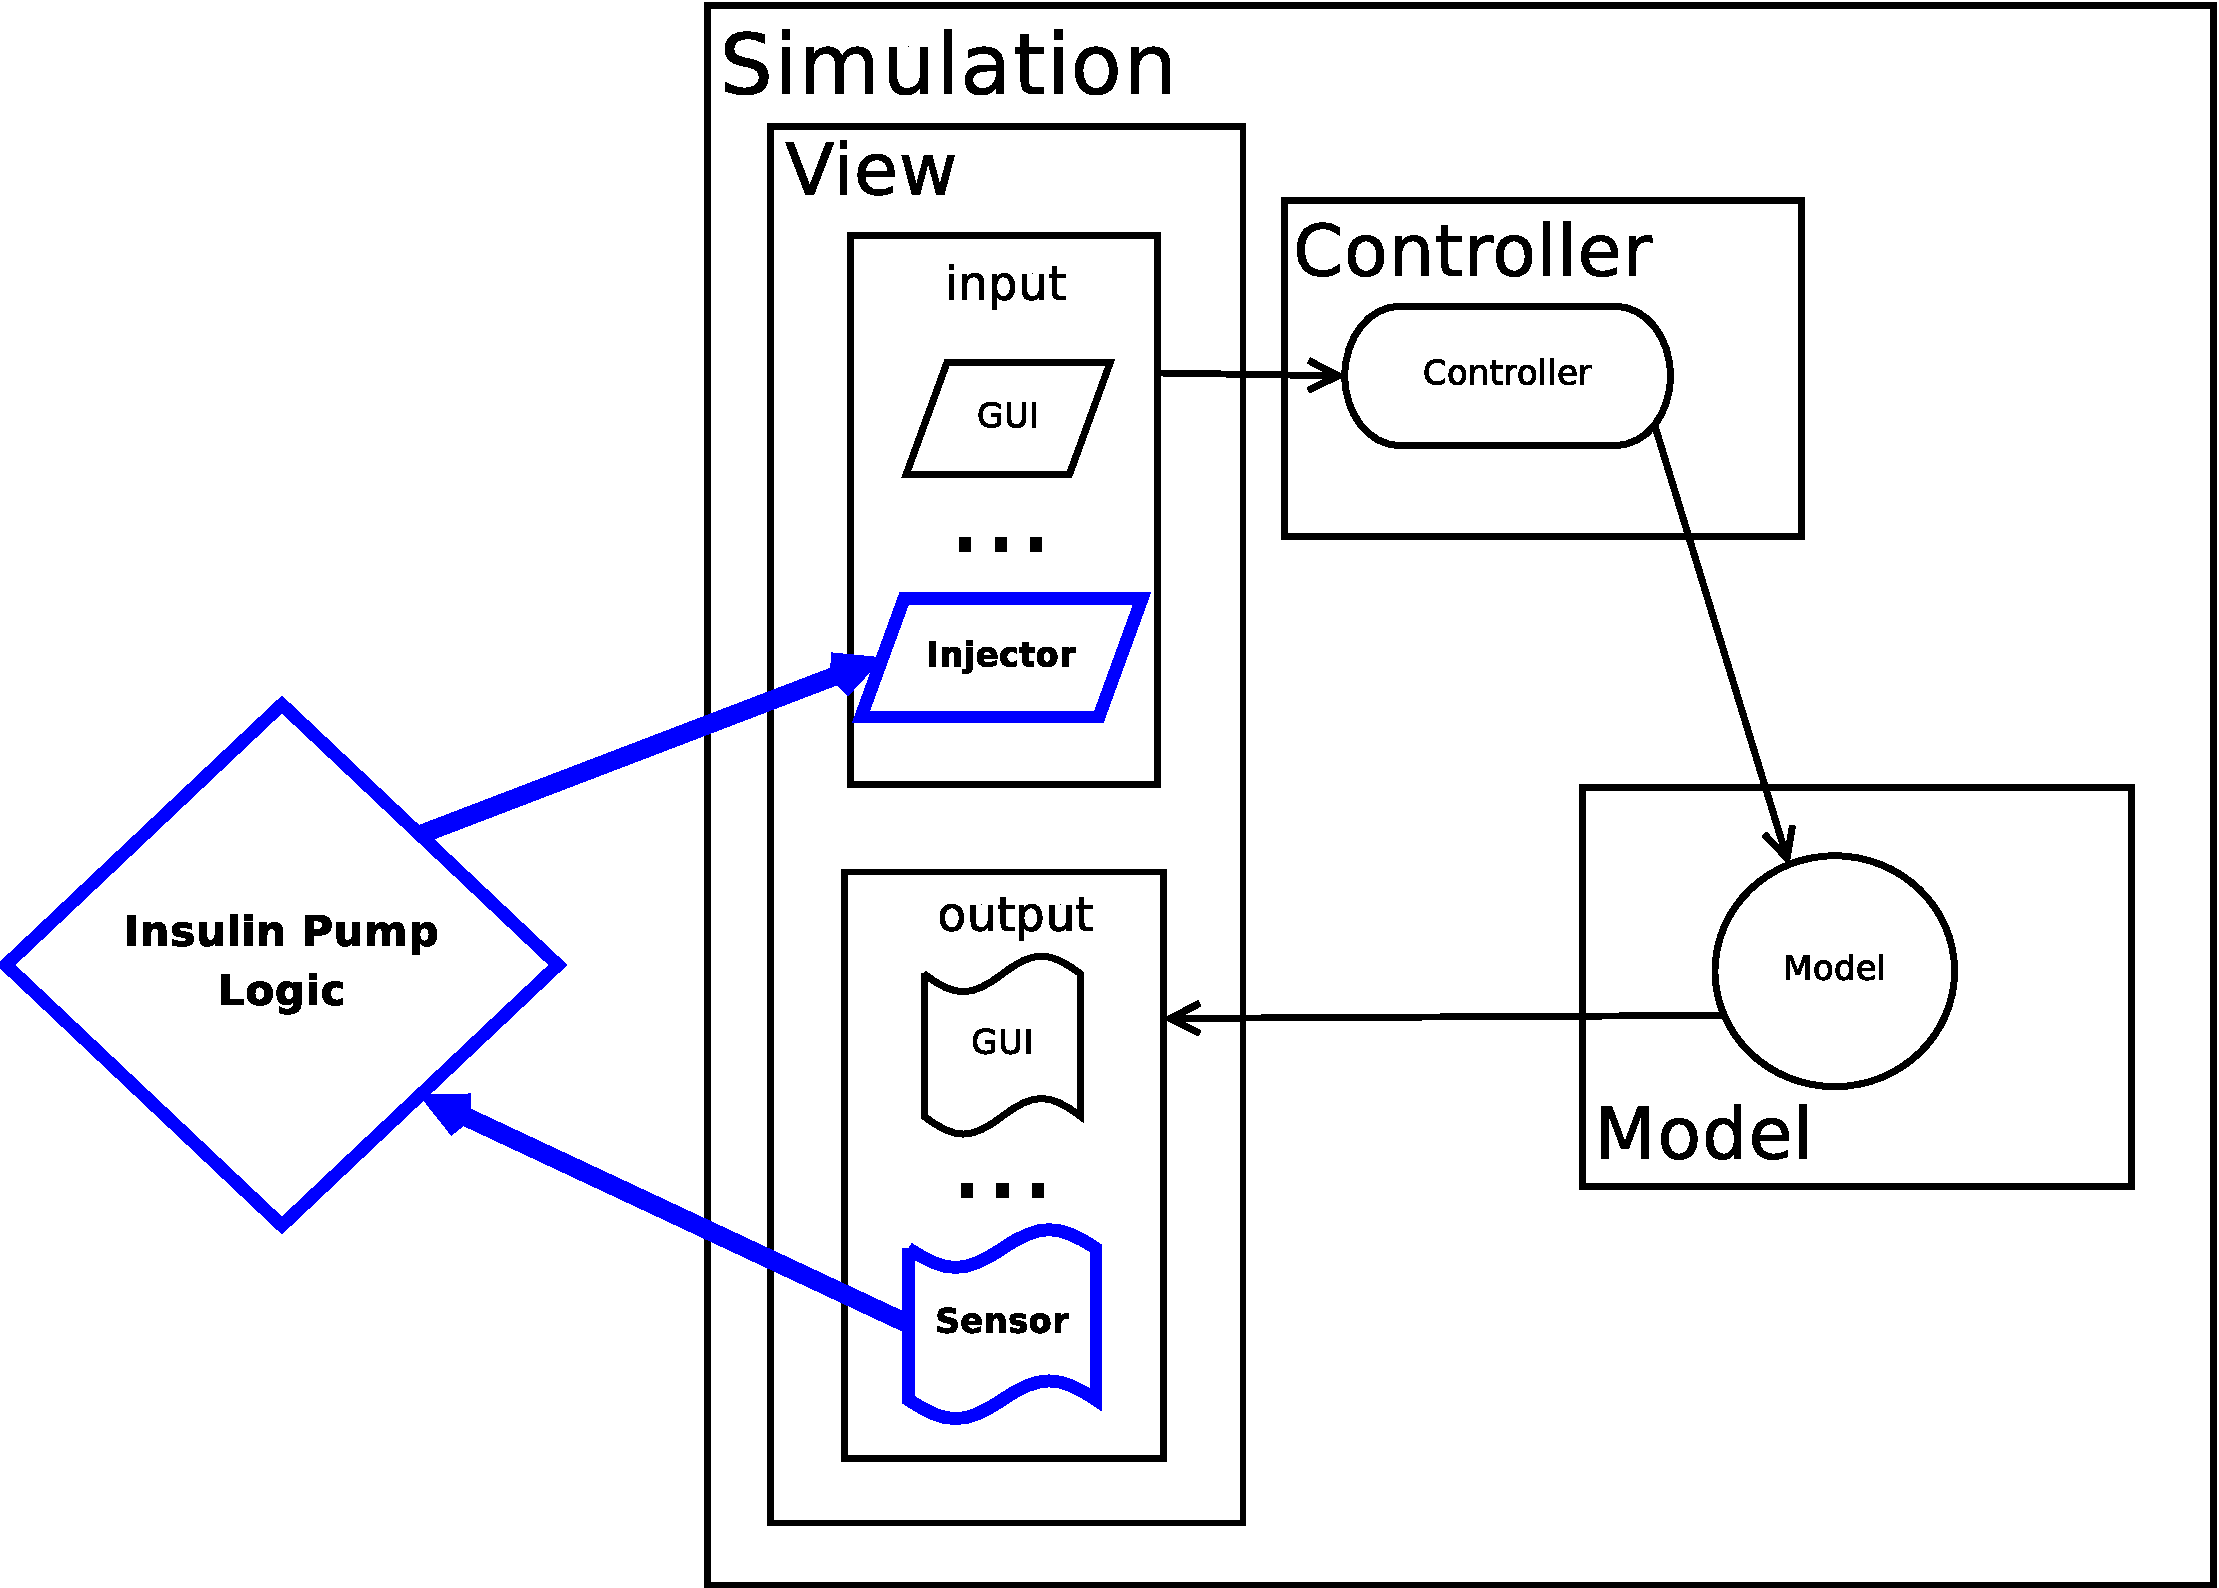
\includegraphics[scale=0.39]{images/mvc_insulin_pump}
\caption{Integration of the Insulin Pump into the Body Simulation}
\label{fig:mvc_insulin_pump}
\end{figure}

\chapter{Conclusion}

\section{Summary}
After having collected all requirements for this project the estimation of the insulin pump project was done by COCOMO 2.\\
The most challenging part of the project was the research. Therefor the project group was divided into three groups to research and implement Diabetes, Food and Insulin.
\\ \\
Diabetes has two types. Only for Type 1 injecting insulin is more common. In Type 1, the body does not produce insulin. And generally diagnosed in children and young adults. There is no known cure for Type 1. People who have diabetes Type 1 have to measure blood glucose level and inject insulin to their body. Their treatment must continue in life-time. The average glucose level, close to normal, is 80-120 mg/dl, 4-6 mmol/l. 600 mg/dl 30 mmol/l level is usually a deadly level for blood glucose. In implementation the following formula was used: for 1 unit of carbonhydrate 1/12 units of insulin needed.\\
There are two major indexes called "Glycemic index" and "Glycemic Load" for Food. 
For simplicity Food is roughly splitted up into three groups according to the indexes in the implementation. These are high Glycemic(acts fastly), moderate Glycemic(intermediate), low Glycemic(acts slowly). Because there are no mathematical models available, rough estimates were made. \\
Insulin is a hormone which is normally produced in the pancreas. Insulin decreases the blood glucose level which is increased by glucagon and some other hormones.  So many types of insulin are existing nowadays. Most commons are: "Insulin analogs (rapid-acting)", "Regular insulin(short-acting)", "Semilente insulin (intermediate-acting)", "Ultralente insulin (long-acting)", "Insulin glargine/ detemir", "Mixture of NPH and regular insulin", "Mixture of semilente and ultralente". The insulin level differs according to the patients. 
\\ \\
For the simulation the tree groups also implemented their parts of simulation. Diabetes module needed to simulate insulin production of ill pancreas. Food module simulated the food types that are discussed. Insulin module took care only of the three types of insulin injections Rapid-Acting, Short-Acting, Long-Acting insulin. \\ 
Finally during the body simulation all modules of the insulin pump were combined. Inputs of body simulation are food and insulin. Outputs are glucose and insulin values over time. 

\section{Conclusion}
The simulation of the insulin pump has been a very interesting task. \\
During this project work we were able to make new experiences concerning project work: after having collected all important requirements the design model of the specification, the design itself, risk analysis, implementing and testing was developed. Furthermore we were able to increase our skills by using different tools for the project estimation. \\
Having the results of the analysis phase on our mind we came to two conclusions:
\begin{itemize}
	\item It is not possible to design / simulate all requirements of the insulin 
			pump in the given time. 
	\item We have to form subgroups that concentrate each on one of the behavioural 
			models, food, insulin and diabetes.
\end{itemize}

So we had to point out the most important functions and order them due to their project priorities. \\
The decision to use patterns like the observer pattern or the model view controller concept helped us to split up the group work easily on the one hand. On the other hand an abstract version of the system could be produced that further implementations can be added without any problems. \\ 
So far we have developed a simulation of a basic insulin pump due to the aspect of time. There are many aspects that have to be taken under consideration before creating a "real" insulin pump. These aspects can be found in the chapters "Further thoughts" or "Future". \\ \\
All in all this project gave us the opportunity to get some deeper knowledge and experience in project work. 


\section{Future}
Maintaining tight control over blood-sugar levels is a daily challenge for people with Diabetes. It requires constant monitoring and multiple insulin injections each day. In our Insulin pump project we can use injectable drug, high glucose levels and automatically dispenses insulin on demand. As glucose levels drop off, the drug stabilizes, trapping insulin until the next glucose spike. Such a drug may cut down the number of insulin injections required to once a day.
In our Insulin Pump Project, drug may also reduce the risk of hypoglycemia, a potential hazard associated with current diabetic therapies. It will find with any person taking insulin that the most dangerous risk is accidental overdose, or not being able to predict how blood sugar will swing after a meal. In our project from a treatment standpoint, Insulin pump would eliminate the risk of dangerously low blood sugar.
\\ 
Diabetes patients currently take insulin pens and traditional syringes, which deliver a single dose of the drug, or insulin pumps, which provide continuous low doses. Throughout the day it may deliver insulin during periods when it's not needed.
\\ \\ 
Before starting clinical trials, we have to avoid side effects of insulin, which can be dangerous. To calculate side effects of our Insulin Pump we have to transmit our source code to physical implementation. Implementation side is so costly that's why before the implementation we can test our system by using some formal methods to already avoid some faults before "real" tests can be started. If  we get safe and reliable results we can go on with further steps. Besides we have to compare our products with our competitors and check -even if our system will be working correctly- if it is not acceptable or if it is under the marketplace. Then we have to reconsider our requirements. In the end -if we are confident that our product is achieving our demands- we can go on with the implementation process to make a prototype of our product. For prototyping of products it is important to make a trial with fake testers and if there are problems concerning the requirement diagram and it is impossible to understand without making a prototype we have to make a trail for this too.
\\ \\
If all the test and data are reliable, we can make a trial with real testers. If this test can be acceptable and safe then our products can be ready to send in assembly line.    

\section{Thank You}
Finally we want to thank our professor, Prof. Dr. M. Wagner, for all the support during this project work.


        
\end{document}
